\section{Initial Analysis}
To begin the analysis, simple plots were made to look at the sensor data over time. Immediately, it was found that the temperature data is quite poor! The resolution of the ADC is evident in the discrete steps that the temperature takes. Figure \ref{fig:BadTemp} shows an example of the temperature data.
\begin{figure}[h!]
\centering
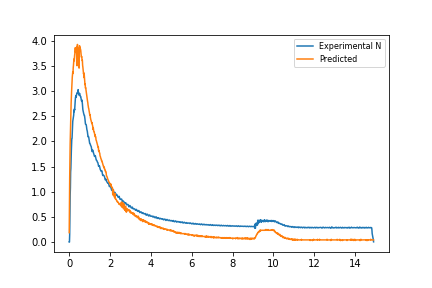
\includegraphics[scale=.5]{Figures/ExampleTemp}
\caption{Example plot of the temperature over time for a trial}
\label{fig:BadTemp}
\end{figure}
The limited resolution of the ADC can be seen quite clearly. However, this is not terribly problematic and several things can be done to smooth the curve. A function from the Pandas Python library that handles smoothing well was used to compensate for this. It uses a moving averages method. The smoothed plot is shown in Figure \ref{fig:SmoothedTemp}.
\begin{figure}[h!]
\centering
\includegraphics[scale=.5]{Figures/SmoothTemp}
\caption{Example plot now smoothed}
\label{fig:SmoothedTemp}
\end{figure}
There are additional problems that come with smoothing data, though. The total number of points is typically reduced and therefore all of the data that is going to be used must then be smoothed by the same factor. Also, the data is shifted to the left as can be seen from Figure \ref{fig:BadTemp} and \ref{fig:SmoothedTemp}. Alternatively, a function could be fit to the data and this would allow the possibility of a continuous data set. For now though, there are bigger problems with the data recorded. Figure \ref{fig:BothTemps} shows the two different temperature data sets plotted against time for one of the trials. 
\begin{figure}[h!]
\centering
\includegraphics[scale=.5]{Figures/TwoSmoothedTemps}
\caption{Smoothed $T_c$ and $T_e$ plotted with time for one of the trials}
\label{fig:BothTemps}
\end{figure}
It can be seen immediately that at some point the $T_c$ line drops below the $T_e$ line. Looking back at Equation \ref{eq:RelevantNozzleForce} this is troublesome. This means that $\left(1-\frac{T_e}{T_c}\right)<0$ giving an overall negative sign under the square root. Obviously the force produced is not imaginary, so either the data collected for these temperatures is not representative of the actual variables or the theory is wrong. It is obvious that the former is the problem for several reasons. The first is that the $T_c$ variable represents the temperature directly before the converging section of the nozzle. $T_e$ is the temperature of the exit plane of the nozzle. The two thermocouples are not placed in these regions. Admittedly, there was not enough attention when inspecting the theory to develop the experiment. Under normal circumstances some simple changes would be made and new data would be taken, however due to the closure of the university nothing can be done about collecting new data. Because of this we will proceed with what analysis can be completed and use a more general approach to characterizing the CGT. First, the predicted force is plotted with the experimental force in Figure \ref{fig:FirstThrust}. 
\begin{figure}[h!]
\centering
\includegraphics[scale=.5]{Figures/FirstAttempt}
\caption{First attempt at plotting the thrust and predicted thrust against time}
\label{fig:FirstThrust}
\end{figure}
As expected, segments where the force is undefined due to a runtime error in the Numpy Python package being used for the square root function.
\section{Attempt at Reconciliation}
The most obvious way to resolve the negative sign is to include an absolute value around the problematic term. This solves the runtime error, but is unfounded. The optimum nozzle expansion ratio should have the largest thrust production, but  $T_e's$ dependence on the exit area is essentially removed on the expansion ratio in doing this. This means the thrust will be highest for the value which has the greatest expansion ratio which is geometry O4. This can be seen in Figure \ref{fig:FirstThreeCurves}. Several trials have been plotted there and included the predicted force according to Equation \ref{eq:RelevantNozzleForce}.
\begin{figure}[h!]
\centering
\includegraphics[width=6.5in]{Figures/FirstThreeCurves}
\caption{Several trials thrust curves plotted with the predicted thrust}
\label{fig:FirstThreeCurves}
\end{figure}
O4 is indeed the largest thrust curve. Also, in viewing these thrust curves it is important to recognize the predicted force is the predicted force per unit mass, but the actual curve is per some different mass value. However, the unit for the mass can be set to some convenient unit and be compared through all the data. This won't change the actual analysis and design conditions.\\
Tacking on an absolute value will not only fail to resolve the issue here but it is also unfounded. The next thought is to solve for $T_e$ in terms of the other available variables. It turns out that $T_e$ can be put in terms of $T_c,\ P_c,\ A_e,\ \rho_c,\ and\ w$. Unfortunately, there are several problems with this. The first is that the change in mass, the mass flow rate, was only measured as an initial and final value. Meaning the total mass used throughout the experiment is known, but the mass flow rate throughout is not. For now, the assumption will be made that the mass flow rate is constant.\footnote{Later, it will be seen this is not the case.} Next, as can be seen from Equation \ref{eq:ExitTemp} $T_e$ cannot be solved algebraically. It is not difficult to solve for it computationally though. 
\begin{equation}\label{eq:ExitTemp}
T_e = T_c\left[\frac{\gamma -1}{2\gamma P_c \rho_c} \left(\frac{w}{A_e}\right)^2\left(\frac{T_c}{T_e}\right)^{\frac{\gamma+1}{\gamma-1}}+1\right]^{-1}
\end{equation}
The simplist method is to use the relaxation method as described in \cite{newman}. The process is to iterate the equation by plugging in $T_e=1$ on the right side, finding a new value for $T_e$ on the left side, substituting this value back into the right side, and so on. $T_e$ should converge to a value and that is the solution for $T_e$. Using this method, I've made the same plots in Figure \ref{fig:SecondThreeCurves} as in Figure \ref{fig:FirstThreeCurves}.
\begin{figure}[h!]
\centering
\includegraphics[width=6.5in]{Figures/SecondThreeCurves}
\caption{Several trials thrust curves plotted with the predicted thrust}
\label{fig:SecondThreeCurves}
\end{figure}
The similarity between the two figures is quite apparent. At first glance, they nearly look the same, but looking at the far right plot the theoretical curve can be seen to be different from the other. The reason for this is because the assumption made about the mass flow rate being constant through time was naive. The mass flow rate, at any point $x$  can be defined by Equation \ref{eq:MassFlow}.
\begin{equation}
w_x=A_x v_x \rho_x
\end{equation}
Both the velocity and density of the gas have dependence on pressure and temperature so $w$ is \textit{not} constant with respect to time. That is not to say it is not constant at any given time throughout the entire system, however. If $T_e$ is not represented correctly it is clear that the result is that the nozzle with the largest expansion ratio is predicted to function best because of Equation \ref{eq:RelevantNozzleForce}'s dependence on $A_e$. \\
Specific impulse values for the experiment can technically be determined. Unfortunately, this doesn't tell much because the theoretical values cannot be calculated for the same reasons as the force. Additionally, it is not ideal to look at the specific impulse over the entire experiment because the temperature and pressure are so transient. Determining these values is a simple trapezoidal sum over all time for the force data and division by the change in mass over the time of the experiment. These values are tabulated in Table \ref{table:Isps}. $I_{sp,1}\ and\ I_{sp,2}$ are the specific impulse for trials 1 and 2 of a geometry. 
\begin{table}[!h]
\centering
\resizebox{\textwidth}{!}{%
\begin{tabular}{
>{\columncolor[HTML]{C0C0C0}}c 
>{\columncolor[HTML]{EFEFEF}}c 
>{\columncolor[HTML]{EFEFEF}}c 
>{\columncolor[HTML]{EFEFEF}}c 
>{\columncolor[HTML]{EFEFEF}}c 
>{\columncolor[HTML]{EFEFEF}}c 
>{\columncolor[HTML]{EFEFEF}}c }
$Geometry$ &
  \cellcolor[HTML]{C0C0C0}$I_{sp,1}\ (s)$ &
  \cellcolor[HTML]{C0C0C0}$I_{sp,2}\ (s)$ &
  \cellcolor[HTML]{C0C0C0}$Avg.$ &
  \cellcolor[HTML]{C0C0C0}$\%Diff.\ T$ &
  \cellcolor[HTML]{C0C0C0}$\%Diff.\ M$ &
  \cellcolor[HTML]{C0C0C0}{\color[HTML]{000000} $\epsilon$} \\
N  & 61 & 54 & 58 & 14 & 6  & {\color[HTML]{000000} 1.00}  \\
U4 & 58 & 44 & 51 & 24 & 16 & {\color[HTML]{000000} 1.25}  \\
U3 & 34 & 53 & 43 & 36 & 29 & {\color[HTML]{000000} 1.64}  \\
U2 & 63 & 60 & 61 & 8  & 1  & {\color[HTML]{000000} 2.07}  \\
U1 & 34 & 63 & 48 & 28 & 21 & {\color[HTML]{000000} 2.56}  \\
O  & 58 & 37 & 47 & 29 & 22 & {\color[HTML]{000000} 6.50}  \\
O1 & 59 & 60 & 59 & 12 & 3  & {\color[HTML]{000000} 10.23} \\
O2 & 51 & 48 & 49 & 26 & 19 & {\color[HTML]{000000} 23.04} \\
O3 & 29 & 60 & 45 & 33 & 27 & {\color[HTML]{000000} 40.95} \\
O4 & 45 & 56 & 50 & 25 & 18 & {\color[HTML]{000000} 64.00}
\end{tabular}%
}
\caption{Table including the determined experimental specific impulse values and percent differences when compared to literature values. Also included is the expansion ratio, $\epsilon$ for each geometry.}
\label{table:Isps}
\end{table}%
\nomenclature{$I_{sp,1}$}{Specific impulse for first trial of a geometry}%
\nomenclature{$I_{sp,2}$}{Specific impulse for second trial of a geometry}